\chapter{Phạm vi và hướng phát triển ứng dụng webfuzzer}
Trong phạm vi luận văn tốt nghiệp này, tôi sẽ áp dụng phương pháp kiểm thử fuzzing dưới dạng kiểm thử hộp đen để hiện thực công cụ \textbf{webfuzzer}. Ngoài khả năng tự động hóa cao, việc áp dụng phương pháp này sẽ đem lại nhiều lợi ích khác.
\begin{itemize}
    \item Linh hoạt trong việc kiểm thử nhiều ứng dụng web sử dụng các công nghệ, mô hình, khung thức phát triển phần mềm khác nhau, cũng như cho phép kiểm thử số lượng lớn ứng dụng web trong một khoảng thời gian ngắn.
    \item Đơn giản hóa và chuẩn hóa việc kiểm thử các lỗ hổng bảo mật trên những ứng dụng web có thiết kế cao cấp và phức tạp. Những ứng dụng này thường có số lượng dòng code có thể lên đến hàng nghìn thậm chí hàng triệu dòng, việc kiểm thử mã nguồn đối với phương pháp hộp trắng hoặc hộp xám sẽ khó khăn hơn nhiều.
    \item Dễ dàng đạt được khả năng tự động hóa cao so với việc quét mã nguồn của ứng dụng. Nhìn chung quá trình phát triển công cụ bằng phương pháp này không yêu cầu kĩ năng lập trình cao hoặc những kĩ thuật nhận diện lỗ hổng quá đặc thù.
    \item Chủ yếu tập trung vào việc kiểm thử chức năng của ứng dụng, không quan tâm đến giao diện, hiệu năng hay trải nghiệm người dùng. Điều này giúp ta có mục tiêu rõ ràng và tiết kiệm công sức cho quá trình thiết kế, cải tiến các trường hợp kiểm thử. 
\end{itemize}
Tương tự như trong lĩnh vực kiểm thử phần mềm, việc áp dụng phương pháp kiểm thử fuzzing dưới dạng kiểm thử hộp đen trong quá trình kiểm thử bảo mật ứng dụng web cũng sẽ có một số hạn chế như sau.
\begin{itemize}
    \item Do không nắm được mã nguồn của ứng dụng web nên chiến thuật tốt nhất là ta chỉ nên tập trung kiểm tra những chỗ thường phát sinh lỗ hổng nhất, hoặc "đoán mò" và vượt qua (bypass) cách thức phòng thủ của ứng dụng bằng việc thử sai và làm rối (tampering) dữ liệu kiểm thử.
    \item Số lượng trường hợp kiểm thử kết hợp với các kĩ thuật bypass đã biết là quá lớn, yêu cầu nhiều kinh nghiệm thực tế của người lập trình để chọn lọc và viết ra được một công cụ nhanh và ổn định, tối ưu hóa tài nguyên máy tính và thời gian thực thi. Ta buộc phải đánh đổi thời gian và tài nguyên đó hoặc chấp nhận kiểm thử trên một tập dữ liệu nhỏ hơn chỉ chứa những trường hợp thường gặp nhất.
    \item Phải có hiểu biết sâu rộng về các lỗ hổng bảo mật, đồng thời thường xuyên cập nhật các trường hợp kiểm thử và kĩ thuật tấn công/phòng thủ mới để bổ sung vào công cụ.
\end{itemize}
Hơn nữa, vấn đề đạo đức nghề nghiệp phải luôn luôn được đặt lên trên hết. Trước và trong quá trình kiểm thử ta phải có thỏa thuận với nhà cung cấp ứng dụng web về mục đích và cách thức tiến hành của mình, hoặc, xác định rõ động cơ của bản thân là để phát hiện những lỗ hổng nguy hiểm và sẽ báo cáo lại với nhà cung cấp để họ vá lỗi, tăng cường bảo mật và bảo vệ quyền lợi của người dùng ứng dụng đó. Bên cạnh đó ta cũng cần phải lưu ý về vấn đề pháp lý của mỗi vùng lãnh thổ địa lý hoặc quy định của những nhà cung cấp khác nhau, cũng như trang bị một số hiểu biết nhất định để bảo vệ danh tính và sự riêng tư của bản thân khi tiến hành kiểm thử số lượng lớn các ứng dụng web xuyên quốc gia.\par
Trong quá trình tìm hiểu và so sánh giữa các phương pháp, công cụ kiểm thử bảo mật ứng dụng web hiện tại, chúng tôi nhận thấy sử dụng chức năng \texttt{Intruder} của Burp Suite là phương pháp phù hợp nhất để tự động hóa quá trình phát hiện các lỗ hổng bảo mật ở tầng ứng dụng của các ứng dụng web thông qua thông điệp \acrshort{http}. \texttt{Intruder} là chức năng triển khai tấn công ứng dụng web tự động, mạnh mẽ và dễ cấu hình. Chức năng này có thể được sử dụng thực hiện những cuộc tấn công với phạm vi trải dài từ đơn giản tới phức tạp, từ vét cạn (brute-force) mật khẩu, thư mục ứng dụng web đến phát hiện các lỗ hổng bảo mật web ở tầng ứng dụng bằng phương pháp fuzzing. Hình \ref{fig:send-base-request-1} sau mô tả giao diện chính của chức năng này.
\begin{figure}[H]
    \centering
        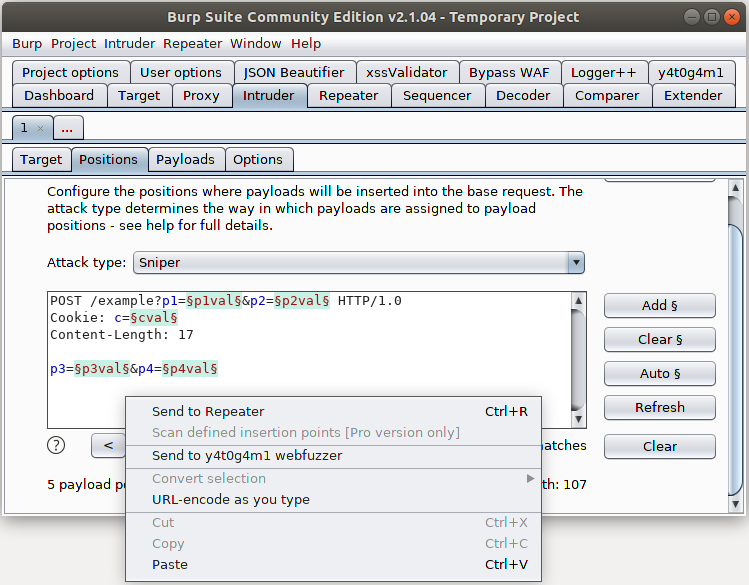
\includegraphics[width=\textwidth,keepaspectratio=true]{images/send-base-request.png}
    \caption{Giao diện chính của chức năng Intruder}
    \label{fig:send-base-request-1}
\end{figure}
Giao diện chính của chức năng này gồm nhiều tab liền kề, mỗi tab được đánh số thứ tự, ứng với một \acrshort{http} request mẫu (base request) cần kiểm thử. Mỗi tab này gồm 4 tab phụ được mô tả như sau.
\begin{itemize}
    \item \textbf{Target} chứa thiết lập địa chỉ IP:port của ứng dụng web mục tiêu.
    \item \textbf{Positions} chứa những thiết lập của request mẫu cần kiểm thử, bao gồm các vị trí truyền tham số và kiểu tấn công.
    \item \textbf{Payloads} chứa các thiết lập liên quan đến tập payload kiểm thử. Tập payload này có thể được nhập từ tập tin trên máy, hoặc được sinh ra bằng một số phần mở rộng khác của Burp Suite, kèm theo các phương pháp tiền xử lí và encode payload thường dùng.
    \item \textbf{Options} chứa những thiết lập liên quan khác trong quá trình tấn công như thời gian chờ, các chuỗi và biểu thức chính quy để so trùng trên \acrshort{http} response trả về,...
\end{itemize}
Nhìn chung, chức năng này sử dụng cặp kí tự ``§'' để đánh dấu vị trí thay thế payload vào request mẫu để tạo thành requets kiểm thử, cụ thể việc sử dụng các danh sách payload và cách thức thay thế payload vào request mẫu như thế nào phụ thuộc vào kiểu tấn công của chức năng \texttt{Intruder}, gồm có \texttt{Sniper, Battering ram, Pitchfork} và \texttt{Cluster bomb}. Kiểu tấn công chúng tôi thường sử dụng nhất trong quá trình fuzzing bằng chức năng này là \texttt{Sniper}. Kiểu tấn công này chèn lần lượt từng payload trong danh sách vào từng vị trí thay thế payload trong request mẫu, do đó tổng số request kiểm thử được hình thành bằng tích số lượng payload nhân với số vị trí chèn payload trong request mẫu. Chúng tôi định ra hướng phát triển ứng dụng webfuzzer, hiện thực lại gần như đầy đủ chức năng \texttt{Intruder}, sử dụng kiểu tấn công \texttt{Intruder} vì những khuyết điểm của ứng dụng Burp Suite như sau.
\begin{itemize}
    \item Việc kiểm thử một request mẫu với nhiều loại lỗ hổng khá phiền phức, người dùng phải lần lượt sao chép các cấu hinh kiểm thử cần thiết vào tab chứa request mẫu. Do đó, nhu cầu định ra một cấu hình kiểm thử mặc định rồi dùng để kiểm thử các request mẫu với nhiều lỗ hổng, cộng với một giao diện trực quan, thân thiện với người dùng hơn, là cần thiết.
    \item Burp Suite không tự động thực thi yêu cầu kiểm thử tiếp theo sau khi hoàn thành yêu cầu hiện tại. Do đó việc xây dựng một ứng dụng kiểm thử xoay quanh các yêu cầu kiểm thử là cần thiết. Việc này giúp quản lý và phân phối tài nguyên máy tính hợp lý hơn, người dùng có thể kiểm soát một lúc có bao nhiêu yêu cầu kiểm thử đang thực thi, tự động thực thi những yêu cầu kiểm thử đã tạo trong thời gian nhàn rỗi, đồng thời cắt giảm thời gian thực hiện các thao tác lặp đi lặp lại của họ so với sử dụng Burp Suite.
    \item Ứng dụng có thể dễ dàng được triển khai ứng dụng kiểm thử ở các dịch vụ cung cấp máy chủ ảo hóa (virtual private service - \acrshort{vps}. Việc kiểm thử bằng Burp Suite trên máy tính cá nhân (đặc biệt là tính năng \texttt{Intruder}) tiêu tốn khá nhiều tài nguyên máy tính, cản trở công việc, dẫn đến nhu cầu tách riêng chức năng này để triển khai trên một máy chủ độc lập. Việc này cũng giúp tránh được nguy cơ địa chỉ IP của máy tính cá nhân bị block theo vùng địa lý hoặc bởi các chính sách kiểm soát lưu lượng truy cập bởi ứng dụng web mục tiêu do gửi quá nhiều request đến trong một khoảng thời gian ngắn, giúp người kỹ sư kịp thời định ra phương hướng khác để tiếp cận mục tiêu.
    \item Việc lưu trữ kết quả kiểm thử ở Burp Suite cần phải được làm bằng tay, dẫn đến nhu cầu cần có một cơ sở dữ liệu để lưu trữ, hệ thống hóa những điểm cuối ứng dụng web có lỗ hổng kèm theo bằng chứng khai thác được lỗi trong quá trình kiểm thử tự động. Việc xây dựng một cơ sở dữ liệu như webfuzzer cũng là tiền đề để mở rộng ứng dụng trên lĩnh vực do thám (reconnaissance) các ứng dụng web mục tiêu trong tương lai.
    \item Việc xây dựng một ứng dụng web để kiểm thử thay vì sử dụng Burp Suite ở máy tính cá nhân còn giải quyết được nhu cầu làm việc chung và chia sẻ dữ liệu kiểm thử của nhiều người trong cộng đồng, hay hẹp hơn là tổ chức, công ty, thay vì chỉ một cá nhân đơn lẻ. Nhiều người có thể trực tiếp đóng góp vào cơ sở dữ liệu và truy vấn thông tin bằng cách sử dụng ứng dụng webfuzzer thay vì Burp Suite ở máy tính cá nhân.
\end{itemize}